\chapter{Preliminaries}
\label{chap:preliminaries}

In this chapter we provide background information in order to understand the previous work done in this field that is introduced in Chapter \ref{chap:related-work}.
We will further rely on the knowledge provided in this chapter when describing the data collection an processing in Chapter \ref{chap:data} as well as when constructing the experimental setup in Chapter \ref{chap:setup}.
We rely on the reader to be patient while reading this chapter as the interplay between the introduced components may not be immediately obvious be will become clear later in the report when the components come to use.
At first, the concept of the previously introduced order book is described in greater detail, as this serves as the data structure for the collected historical data.
Subsequently, a simplified match engine is described with which we will emulate a local broker that can match orders given the historical order book.
An introduction to the properties of a time series is then introduced as the order book underlies its principles.
Furthermore, reinforcement learning is introduced, whereas we declare the differences to other machine learning techniques, followed by a detailed explanation of all its components.
Finally, deep reinforcement learning is introduced as an extension to the previously described reinforcement learning principles.

\section{Order Book}

Traders post orders in a limit order book in order to state their intention to buy (respectively sell) a given asset, as described in Section \ref{sec:problem-statement}).
Orders listed in the limit order book implicitly provide so called \textit{liquidity} to the market as other traders can consume these offerings by posting an order with the equivalent price to sell (respectively buy) the asset.
%The former group of traders is known as \textit{liquidity traders} and is rewarded by a broker with lower fees than the latter group as they provide liquidity and therefore make the market alive (hence why the feed is known as \textit{maker fee}).
%The latter group who consumes the orders of the former group implicitly takes out liquidity of the market and therefore has to pay an increased fee to do so (hence why the feed is known as \textit{taker fee}).

This section introduces the most popular order types with which a trader can post their offerings into a limit order book.
We will learn with which type a trader can ensure to provide liquidity to the market and benefit from lower fees and with which type the trader can state the wish to immediately buy or sell assets and implicitly take liquidity from the market.
Furthermore, the characteristics an historical order book that is filled with orders from traders is explained as this will come handy when the match engine is explained in the following section.

\subsection{Orders}
\label{sec:orders}

As indicated by the name, an order is an order to buy or sell a stock.
There are various types of orders which determine how the order that is placed should be executed by the exchange.
In this section we provide information about the two most common types, namely the \textit{limit order} and the \textit{market order},
We define the indication on whether to buy or sell as the \textit{Order Side},
\begin{equation}\label{eq:order-side}
    OrderSide=\{Buy, Sell\}
\end{equation}
\\
Before we define the order types in greater detail, we conclude what is said above and define the \textit{Order} as,
\begin{equation}\label{eq:order}
Order=\{Order_{Limit}, Order_{Market}\}
\end{equation}

\subsubsection{Limit order}
\label{sec:limit-order}

A limit order implies the attempt to buy or sell a stock at a specific price or better,
\begin{equation}\label{eq:order-limit}
    Order_{Limit}=(side, quantity, price_{Limit})
\end{equation}
, where $side \in OrderSide$, $quantity \in \mathbb{R^+}$ and $price_{Limit} \in \mathbb{R^+}$.
\\
\\
A buy limit order can only be executed at the limit price or lower, and a sell limit order can only be executed at the limit price or higher \cite{sec-limit-order}.
More precisely, in case of a buy order and if the best price on the opposing side of the book becomes lower or equals (respectively higher or equals, in case of a sell order), the broker will match those two orders, resulting in a \textit{trade}.
The disadvantage of this order type is that there is no guarantee whether the order gets executed.
In case no order on the opposing side appears, the order remains (possibly forever) unexecuted.

\subsubsection{Market order}
\label{sec:market-order}

A market order implies the attempt to buy or sell a stock at the current market price, expressing the desire to buy (respectively sell) for the best available price. Therefore,
\begin{equation}
Order_{Market}=(side, quantity)
\end{equation}
, where $side \in OrderSide$ and $quantity \in \mathbb{R^+}$.
\\
\\
The advantage of a market order is that as long as there are willing buyers and sellers, the execution of the order is almost always guaranteed. \cite{sec-market-order}
The disadvantage is the price you pay when your order is executed.
Market orders are executed by starting from the best price of the opposing side, then traversing down the book as liquidity is consumed. 
Hence, market orders tend to become expensive, especially for large orders.

\subsection{Characteristics}
\label{sec:ob-characteristics}

Figure \ref{fig:intro-orderbook} shows a real world example of a limit order book; in this case the snapshot was taken from a known crypto-currency exchange.
Being precise, this is the \textit{state} of an order book at some time $t$ and shows the current offerings (in form of limit orders, see \ref{sec:limit-order}) from participants at this moment in time (we neglect the possibility that the state might have been changed during the data sending process). 
Hence, we refer to it as an \textit{order book state (OS)}.
We refer to the \textit{order book (OB)} that is used in this project as a recorded history of order book states.
\begin{equation}\label{eq:order-book}
OB=OS_1, ... OS_n
\end{equation}
As we can see, every such state holds entries on the buyer and seller side which change in their \textit{price} and \textit{amount}.
To each such row, which can be formed by participants who submitted limit orders of some amount at the same price level, we refer to as \textit{order book entry ($OE_{s_l}$)} of the side $s$ at level $l$.
\begin{equation}
OE_{s_l}=(count, price, amount)
\end{equation}
, whereas $count \in \mathbb{N}$, $price \in \mathbb{R^+}$ and $amount \in \mathbb{R^+}$.
As a result, the order book state is a sequence containing order book entries for each \textit{side} (buy and sell) and a time stamp $ts$ of the state,
\begin{equation}\label{eq:order-book-state}
OS=(ts, OE_{b_1}, ..., OE_{b_n}, OE_{s_1}, ..., OE_{s_n})
\end{equation}
\\
\begin{figure}[H]
    \centering
    \makebox[\linewidth]{
        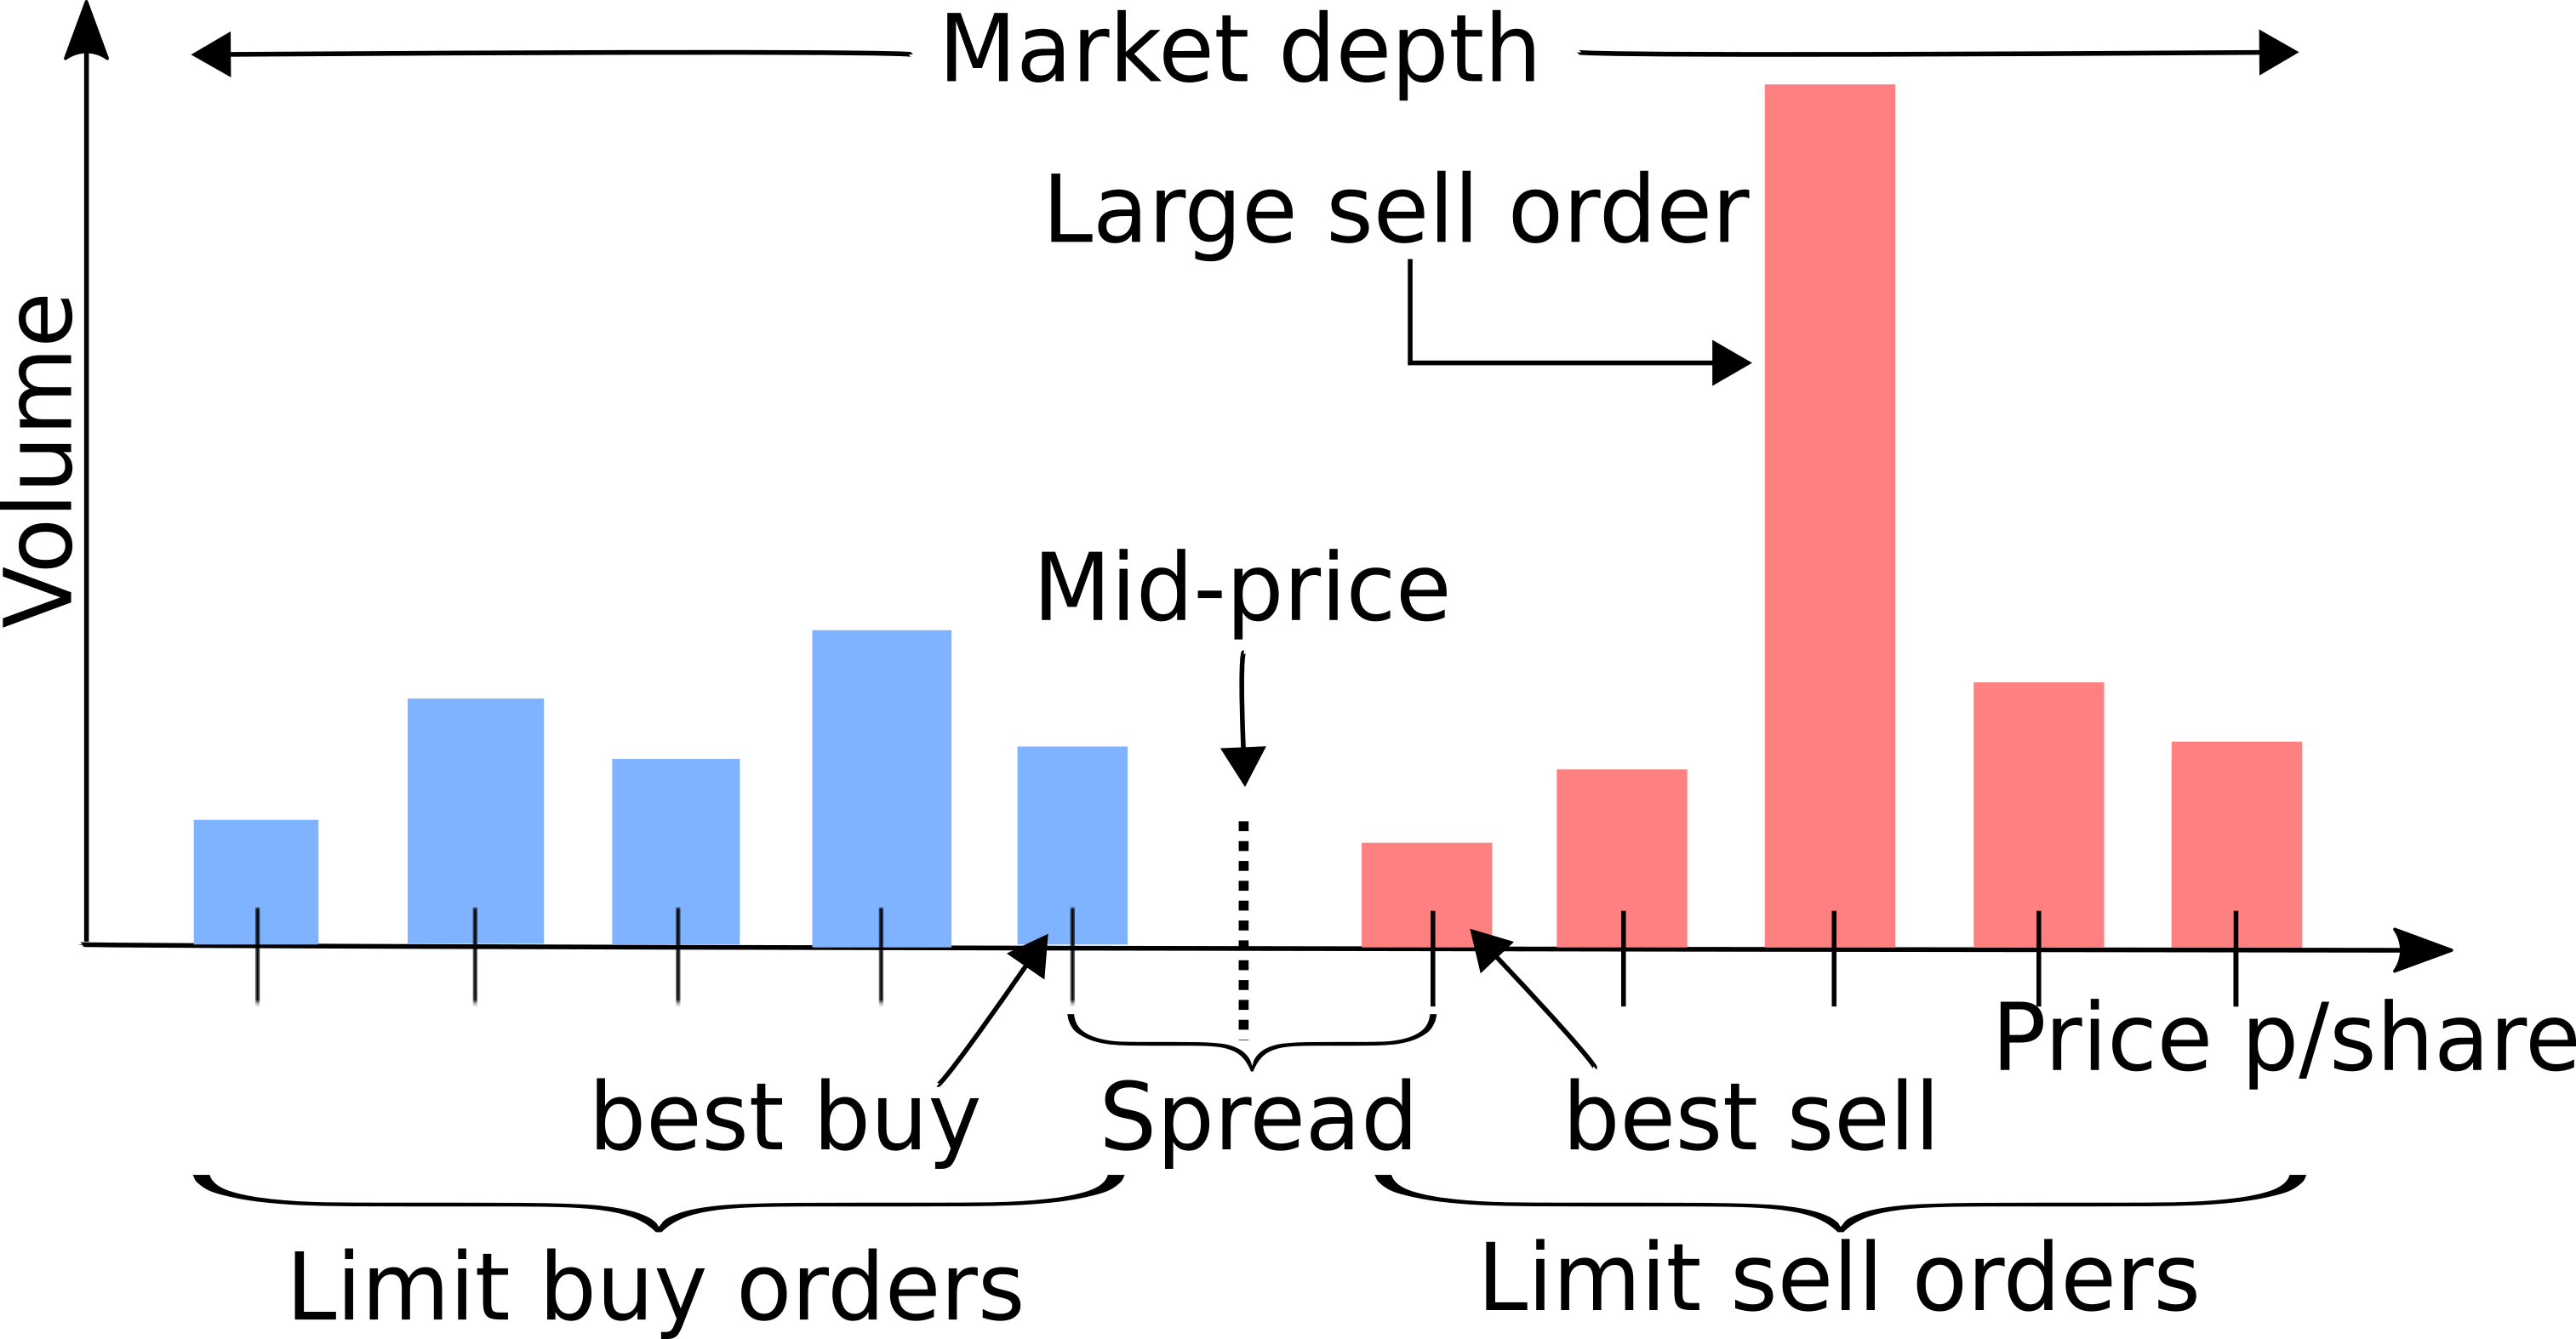
\includegraphics[width=10cm]{lob-simple.png}
    }
    \caption{Figure taken from \cite{miranda}. Simplified limit order book and provides understanding of some characteristics.}
    \label{fig:orderbook-simple}
\end{figure}
\hfill
\\
Figure \ref{fig:orderbook-simple} illustrates a simplified order book, from which we can derived definitions.
The \textit{limit level} specifies the position of an order book entry within the side of an order book state and the so-called \textit{market depth} corresponds to how deep in the order book buyers and sellers have listed offerings.
A deep order book therefore indicates a large range of limit levels.
The term \textit{volume} can relate to the total volume traded over a given time horizon, or can indicate the sum of amounts of what is currently offered to a certain price.
Considering the sides of the order book, a \textit{bid} refers to a price on the buyer side and the \textit{best bid} represents the highest price for which someone is willing to buy a given asset.
The best bid appears as the first order book entry on the buyer side, closest to the spread.
Contrarily, an \textit{ask} refers to a price on the seller side and the \textit{best ask} represents the lowest price for which someone is willing to sell a given asset. 
The best ask appears as the first order book entry on the seller side, closest to the spread.
Consequently, the \textit{market price} is the average between the best bid and best ask price and the \textit{spread} indicates the difference between the best bid and best ask.

The most recent price on which a buyer and seller agreed upon to trade a security is known as \textit{quote}.
In an \textit{order driven market}, liquidity is a synonym for the ease of trading.
\textit{Liquidity} stands for the amount provided by parties of the opposing side and is what effectively enables one to buy and sell securities.
That is achieved by submitting limit orders which are not immediately executed.
A so called \textit{market maker} provides liquidity to the market by posting limit orders which are not immediately executed.
In return, the market maker pays less fees than a market taker, the so-called \textit{maker fee}.
Contrarily, the \textit{market taker} takes liquidity out of the market by posting either market orders or limit orders which immediately execute.
As this is not beneficial to the exchange, the market taker pays a slightly increased rate of fees, known as \textit{taker fee}.

\section{Match Engine}
\label{sec:match-engine}

The \textit{matching engine} is the component which responsible for the process of matching buy and sell orders at a stock exchange, such as \textit{NASDAQ} or \textit{NYSE} as examples of traditional stock exchanges; or \textit{Bitfinex}, \textit{Bittrex}, \textit{Coinbase} as examples of crypto-currency exchanges.
In order to determine the outcome of an order, the trader would typically submit the order to an exchange and either trade on the live market or get access to a test environment, which can be, if existent, still costly.
Consequently, the order is processed at the current market and there is no option to process it on a historical data set in order to determine outcome, had the order been posted at some time $t$ in the past.
For the aforementioned reasons, a \textit{local} match engine is being developed that allows to evaluate the outcome of order placement on a historical order book data set, free of charge.
The local match engine is a key element of the order placement optimization process that ultimately a reinforcement learner will proceed.
The outcome of matched orders will directly affect the reward received by an agent with which it will try to improve its capabilities.

This section first give the definition of a \textit{trade} as a result of two matching orders.
Subsequently, the time horizon as an addition to the previously introduced order types (Section \ref{sec:orders}) is presented with which we can describe the interface of the match engine that will be used throughout the learning process.
Finally the rules of the implementation of the local match engine is provided which explain the mechanics of the matching process.

\subsection{Trade}

In order to understand the purpose of the matching process, which is described in more detail below, we first have to define what a \textit{trade} is.
A trade results when the orders (Eq. \ref{eq:order}) from two parties with opposing order side (Eq. \ref{eq:order-side}) agree on an amount and price to trade their shares.
That is,
\begin{equation}\label{eq:trade}
    Trade=(ts, side, type, quantity, price )
\end{equation}
, where $ts$ is the time-stamp when the participants agreed on the exchange of the products, $side \in OrderSide$, $type \in OrderType$, $quantity \in \mathbb{R^+}$ and $price \in \mathbb{R^+}$.

\subsection{Interface}
\label{sec:match-engine-interface}

This match engine enables the simulation and evaluation of order placement without the need to consult an electronic trading network.
Alongside the order that is sent to the match engine (directly or via an electronic trading network), the user can specify a \textit{time horizon} $H$ indicating how long the order should stay active.
The two most commonly used timing mechanisms are:
\begin{description}
    \item[Good Till Time (GTT): ] The order stays in the order book until a specified amount of time is consumed. \textit{(Some implementations declare the same idea as Good Till Date whereas a date and time is provided which specifies until when the order is valid.)}
    \item[Good-Til-Canceled (GTC): ] The order stays in the order book until the user submits a cancellation.
\end{description}
\hfill
\\
Hence, the match engine exposes an interface that represents a function $match$ which takes any type of an \textit{Order} (Section \ref{sec:orders}) and the time horizon $H$ and returns a sequence of \textit{trade} (Eq. \ref{eq:trade}).
That is,
\begin{equation}
    match : Order \times H \rightarrow Trades
\end{equation}
, whereas $|Trades| \in \mathbb{N}$.
The order is \textit{filled} if the sum of the traded quantity is equal to the amount stated in the submitted order, \textit{partially-filled} if the traded quantity is $> 0$ but not filled and \textit{not filled} otherwise.
\\
\\
\textit{The matching process behaves different, depending on the submitted order type, and is explained in the following paragraph.}

\subsection{Rules}

The rules presented below are, compared to match engines used in electronic trading networks, are rather primitive, yet correct within the subset of its capability.
The rules used by the order matching engine are mainly derived and simplified from \cite{match-engine}:
\begin{enumerate}
    \item Limit orders (defined in Section \ref{sec:limit-order}) may be partially filled or not filled at all in case of absence of parties on the opposing side.
    
    \item Market orders (defined in Section \ref{sec:market-order}) will execute immediately when an opposite order exists in the market.
    
    \item Market orders may be partially filled, at different prices, depending on liquidity in the opposing side of the book.
    
    \item Limit orders are attempted to be matched from the given point in time forward, or in case of a Good Till Time (GTT) for as long as specified.
\end{enumerate}


\subsection{Limitations}

Since the match engine used in this project is a rudimentary implementation for the purpose of simulating and analyzing order execution and placement, it features only a subset a conventional match engine used by electronic trading networks.
That said, the following limitations have to be taken into consideration:
\begin{description}
    \item[Participants:] first and foremost, the match engine is used locally where no other participants are interacting during its use.
    In order to be able to approximate the most likely outcome, historical data serves as a simulation of participants acting in the market.
    While this is valuable real world data, unfortunately it does not cover 1) the possibility of hidden participants entering or 2) leaving the market upon placing an order from our side.
    Participants who would enter the market would likely be in our favour as they would act as potential buyers and sellers and therefore provide liquidity.
    Participants who leave the market would introduce a slight disadvantage as there would be less liquidity.
    Since both parties are absent, we consider our implementation as a good approximation without a major advantage or disadvantage.
    
    \item[Ordering] this match engine is restricted to simulate the matching of only one order from one participant at a time.
    Hence, any type of ordered processing of incoming orders (typically solved with a queuing system) is not supported.
    However, this functionality is also not required for our purposes.
    
    \item[Timing inaccuracy:] occurs when submitting an order with a time horizon (see Section \ref{sec:match-engine-interface}).
    The fact that we rely on historical data and the time stamps of the orders submitted from participants in the past is a limitation when submitting an order over a certain period of time (GTT).
    It can occur that at the end of the period the order would have some time $t$ left (e.g. a few seconds) but the next following order book state is nearer to the future than $t$ would allow.
    We therefore have to abort the matching process early.
    
\end{description}

\section{Order execution and placement}
\label{sec:execution-placement}

Given the understanding of the order book and the match engine, it is obvious that a trader has a variety of options on how to approach a market and fulfill his duties to buy (respectively sell) shares.
Conceptually, the process a trader proceeds involves the following two steps: \textit{order execution} and \textit{order placement}, whereas the latter is the main subject of this thesis.

Many useful definitions which highlight the difficulties related to the order execution domain were stated by Lim et al. \cite{lim2005optimal} and Guo et al. \cite{guo2013optimal}.
Most importantly, \textit{order execution} concerns about optimally slicing big orders into smaller ones in order to minimize the price impact, that is, moving the price up by executing large buy orders (respectively down for sell orders) at once. 
By splitting up a big order into smaller pieces and spreading the execution over an enlarged time horizon, the impact cost can be lessened.
Typically on a daily or weekly basis.
Contrarily, \textit{order placement} concerns about optimally placing orders within ten to hundred seconds.
Placing hereby refers to the setting of the limit level for a limit order as described in Section \ref{sec:limit-order}.
The aim is to minimize the \textit{opportunity cost} which arises when the price moves against our favour.

Literature\cite{nevmyvaka2006reinforcement, guo2013optimal} suggests to use the \textit{volume weighted average price (VWAP)} as a measure of the \textit{return} of order placement and order execution.
That is,
\begin{equation}\label{eq:vwap}
    p_{vwap}=\frac{\sum{v_p*p}}{V}
\end{equation}
, whereas $p$ is the price paid for $v_p$ shares and $V$ represents the total volume of shares.

\section{Time series}

According to the efficient market hypothesis\cite{malkiel1989efficient}, the price of an asset reflects all the information available to the market participants at any give time. 
Given the vast information flow, the natural consequence is that the price of such an asset changes over time.
As we have seen in the previous Section \ref{sec:order-book}, the price of an asset is determined by actions proceeded by traders.
Therefore, the financial markets and particularly the order book are best described over time, namely as a \textit{time series}. 
More precisely, the definition of a time series is an ordered sequence of values of a variable at equally spaced time intervals \cite{intro-timeseries}.
The nature of time series data originated the applications generally known as Time Series Analysis and Time Series Forecasting.
Both of which play an important role throughout this project, and therefore a brief background is provided in this section.

\subsection{Time series analysis}

The analysis of data observed at different points in time leads to problems in statistical modelling and inference. 
More specifically, the correlation of adjacent points in time can restrict the applicability of conventional statistical methods which traditionally depend on the assumption that these adjacent observations are independent and identically distributed. 
A systematic approach by which one attempts to answer the mathematical and statistical questions posed by these time correlations is commonly referred to as time series analysis. 
Therefore, mathematical models are developed with the primary objective to provide plausible descriptions for sample data. \cite{shumway2000time}
%\subsubsection{Random variables}
%
%A collection of random variables indexed according to the order they are obtained in time serves as a representation of the time series. For example, a time series with three data points ($x_1$, $x_2$, $x_3$) can be considered as a sequence of the random variables $x_1$, $x_2$ and $x_3$, where the random variable $x_1$ denotes the value of the first time period, the variable $x_2$ denotes the value for the second time period and $x_3$ denotes the value for the third time period. While graphically plotting the values of random variables, it is conventional to display the random variables on the vertical axis with the time scale as abscissa. \cite{shumway2000time}
%\\
%\\
%One such example of a time series analysis, %that is often times seen in the context of %financial data, is the moving average. 
%
%\begin{equation}
%    v_t=\frac{1}{3}(x_{t-1}+x_t+x_{t+1})
%\end{equation}
%
%Moving average allows to smoothen the %series by averaging the current value and %its immediate neighbors in the past and %future.
%
\\
\\
Some of the time series behaviours, which will be presented within this body of work, may hint that a sort of regularity exist over time.
We refer the notion of regularity using a concept called \textit{stationarity}, as introduced in \cite{shumway2000time}.
\\
\\
A \textbf{strictly stationary} time series is one for which the probabilistic behavior of every collection of values
${x_{t_1}, x_{t_2}, ..., x_{t_k}}$
is identical to that of the time shifted set
${x_{t_1+h}, x_{t_2+h}, ..., x_{t_k+h}}$
for all time shifts $h=0,\pm1,\pm2,...$
\\
\\
A \textbf{weakly stationary} time series, $x_t$, is a finite variance process such that
\begin{itemize}
    \item the mean value function $\mu_t$ is constant and does not depend on time $t$, and
    \item the autocovariance function $\gamma(s, t)$, depends on $s$ and $t$ only through their difference $|s-t|$.
\end{itemize}

Whereas $\mu_t$ is defined as

\begin{equation}
    \mu_{t}=\mathbb{E}(x_t)=\int_{-\infty}^{\infty} x f_t(x) dx
\end{equation}

with $f_t$ being the \textit{marginal density function} \cite{shumway2000time}.
And $\gamma(s, t)$ is defined as
\begin{equation}
    \gamma(s, t)=cov(x_s, x_t)=\mathbb{E}[(x_s-\mu_s)(x_t-\mu_t)]
\end{equation}

for all time points $s$ and $t$.
\\
\\
\textit{Henceforth, we will use the term stationary to mean weakly stationary; if a process is stationary in the strict sense, we will use the term strictly stationary.}

\subsection{Time series forecasting}

In statistics, prediction is a part of statistical inference. 
Providing a means of the transfer of knowledge about a sample of a population to the whole population, and to other related populations is one description of statistics. 
However, this is not necessarily equivalent to the process of predicting over time. 
This process, instead, is known as forecasting and describes the transfer of information across, often to very specific point in, time \cite{wiki-timeseries}.
Hence the problem is defined in \cite{ito1993encyclopedic} as: \textit{forecasting future values $X_{t+h}$ where $h > 0$ of a weakly stationary process ${X_t}$ from the known values $X_s$ where $s \leq t$}. 
The integer $h$ is called lead time or forecasting horizon, whereas $h$ stands for horizon.
\\
\\
Forecasting methods can be classified, according to \cite{chatfield2000time}, into three types: \textit{Judgemental forecasts} produce projections based on intuition, inside knowledge, and any other relevant information.
\textit{Univariate methods} forecast depends on present or past values of the time series on which the forecast is projected.
Finally, \textit{multivariate methods} forecast depends on one or more additional time series variables or multivariate models.
\\
\\
\textit{Over the course of this work, we make use of univariate- and multivariate methods.}

\section{Reinforcement Learning}
\label{sec:reinforcement-learning}

This section first aims to describe what Reinforcement Learning is and highlights its differences to other machine learning paradigms. 
We briefly reason why this particular technique might be an appropriate choice for the task of optimizing order placement. 
Then, a basic understanding about Markov Decision Processes is provided, after which we explain the interaction between the Reinforcement Learning components, followed by a description of their properties.

\subsection{Advantages of end-to-end learning}

\begin{figure}[H]
    \centering
    \makebox[\linewidth]{
        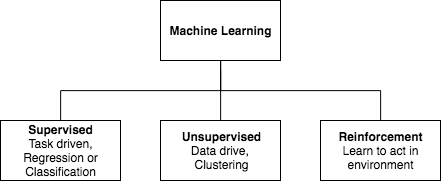
\includegraphics[width=8cm]{ml-rl.png}
    }
    \caption{Categorization of machine learning techniques}
    \label{fig:ml-rl}
\end{figure}

Reinforcement Learning is a specific learning approach in the Machine Learning (see Figure \ref{fig:ml-rl}) field and aims to solve problems which involve \textit{sequential decision making}.
Therefore, when a decision made in a system affects the future decisions and eventually its outcome, the aim is to learn the optimal sequence of decisions with reinforcement learning.

\begin{figure}[H]
    \centering
    \makebox[\linewidth]{
        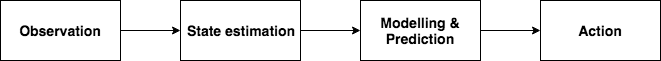
\includegraphics[width=12cm]{rl-pipeline.png}
    }
    \caption{Reinforcement learning end-to-end learning pipeline}
    \label{fig:rl-pipeline}
\end{figure}

For optimizing order placement in limit order books, statistical approaches have long been the preferred choice.
While statistics emphasizes inference of a process, machine learning on the other hand emphasizes the prediction of the future with respect to some variable.
Machine learning paradigms, such as supervised learning, rely on an algorithm that learns by presenting a specific situation provided with the right action to do. 
From there, the algorithm tries to generalize the model.

Contrarily, in reinforcement learning there is no supervision and instead an agent learns by maximizing rewards.
The feedback retrieved while proceeding a task with a sequence of actions might be delayed over several time steps and hence the agent might spend some time exploring until it finally reaches the goal and can updates its strategy accordingly.
This process can be regarded as \textit{end-to-end learning} and is illustrated in Figure \ref{fig:rl-pipeline}.
In abstract terms, the agent makes an \textit{observation} of its environment and estimates a \textit{state} for which it \textit{models and predicts} the \textit{action} to be taken.
Once the action was executed, the agent receives a \textit{reward} and will take this into consideration during during the prediction phases in the future. 
The beauty of which is that an arbitrarily complex process can be regarded as a black box as long as it can take an input from the learner to do its job and responds how well the task was executed.
In our context this implies that we would model the order placement process pipeline whereas the learner improves upon the outcome of the submitted orders.
In addition, for reinforcement learning problems, the data is not independent and identically distributed (I.I.D). 
The agent might in fact, while exploring, miss out on some important parts to learn the optimal behaviour. 
Hence, time is crucial as the agent must explore as many parts of the environment to be able to take the appropriate actions. \cite{rl-demystified}
\\
\\
\textbf{Example:} Since we are working with financial systems, let us assume we want to buy and sell stocks on a stock exchange. 
In reinforcement learning terms, the trader is represented as an \textit{agent} and the exchange is the \textit{environment}.
The details of the environment do not have to be known as it is rather regarded as a black-box.
The agents purpose is to observe the state of the environment: say for example the current price of a stock.
The agent then makes estimates about the situation of the observed state and decides which action to take next – buy or sell. 
The action is then send to the environment which determines whether this was a good or bad choice, for example whether we made a profit or a loss.

\subsection{Markov Decision Process (MDP)}
\label{rl-mdp}

A process such as the one sketched above, can be formalized as a Markov Decision Process.
An MDP is a 5-tuple $(S, A, P, R, \gamma)$ where:
\begin{enumerate}
    \item $S$ is the finite set of possible states $s_t \in S$ at some time step.
    \item $A(s_t)$ is the set of actions available in the state at time step $t$, that is $a_t \in A(s_t)$, whereas $A=\bigcup_{s_t \in S} A(s_t)$
    \item $p(s_{t+1} | s_t, a_t)$ is the state transition model that describes how the environment state changes, depending on the action $a$ and the current state $s_t$.
    \item $p(r_{t+1} | s_t, a_t)$ is the reward model that describes the immediate reward value that the agent receives from the environment after performing an action in the current state $s_t$.
    \item $\gamma \in [0,1]$ is the discount factor which determines the importance of the future rewards.
\end{enumerate}

\subsection{Interaction}

\begin{figure}[H]
    \centering
    \makebox[\linewidth]{
        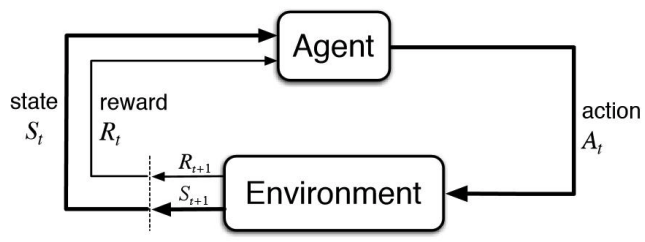
\includegraphics[width=10cm]{rl-overview.png}
    }
    \caption{Figure taken from \cite{rl-demystified}: interaction between a reinforcement learning agent and environment. Illustrating the action taken by the client being in some state which results in some reward and a new state.}
    \label{fit:rl-overview}
\end{figure}
\\
\\
A reinforcement learning problem is commonly defined with the help of two main components: \textit{Environment} and \textit{Agent}.
\\
\\
With the interfaces provided above (Section \ref{rl-mdp}), we can define an interaction process between an agent and environment by assuming discrete time steps: $t=0, 1, 2, ...$

\begin{enumerate}
    \item The agent observes a state $s_t \in S$
    \item and produces an action at time step $t$: $a_t \in A(s_t)$
    \item which leads to a reward $r_{t+1} \in R$ and the next state $s_{t+1}$
\end{enumerate}
\\
\\
During this process, and as the agent aims to maximize its future reward, the agent consults a \textit{policy}, which dictates which action to take given a particular state.

\subsubsection{Policy}

A policy is a function that can be either deterministic or stochastic. 
The distribution $\pi(a|s)$ is used for a stochastic policy and a mapping function $\pi(s) : S \rightarrow A$ is used for a deterministic policy, whereas $S$ is the set of possible states and $A$ is the set of possible actions.
\\
\\
The stochastic \textit{policy} at time step $t$: $\pi_t$ is a mapping from state to action probabilities as a result of the agents experience, and therefore, $\pi_t(a|s)$ is the probability that $a_t=a$ when $s_t=s$.

\subsubsection{Reward}

The goal is that the agent learns how to select actions such that it maximizes its future reward when submitting them to the environment.
We rely on the standard assumption that future rewards are discounted by a factor of $\gamma$ per time-step in the sense that the total discounted reward accounts to $r_1 + \gamma*r_2 + \gamma^2*r_3 + \gamma^3*r_4 + ...)$
\\
Hence we define the future discounted \textit{return} at time $t$ as 

\begin{equation}\label{eq:discounted-return}
R_t=\sum_{i=t}^{T}{\gamma^{i-t}{*}r_{i}}
\end{equation}
, where $T$ is the length of the episode (which can be infinity if there is no maximum length for the episode).
\\
The discounting factor has two obligations: it prevents the total reward from going to infinity (since $0 \leq \gamma \leq 1$), and it allows to control the preference of the agent between immediate rewards and potentially received reward in the future. \cite{rl-demysitifed2}

\subsubsection{Value Functions}

When the transition function of an MPD is not available, model-free reinforcement learning allows the agent to simply rely on some trial-and-error experience for action selection in order to learn an optimal policy.
Therefore, the value of a state $s$ indicates how good or bad a state is for the agent to be in, measured by the expected total reward for an agent starting from this state. Hence we introduce the \textbf{value function}, which depends on the policy the agent chooses its actions from:

\begin{equation}\label{eq:value-function}
V^{\pi}(s)=\mathbb{E}[R_t]=\mathbb{E}[\sum_{i=1}^{T}{\gamma^{i-1}{r_{i}}}]\ \forall s \in S
\end{equation}
\\
Among all value functions there is an \textbf{optimal value function} which has higher values for all states

\begin{equation}\label{eq:optimal-value-function}
V^{*}(s)=\max_{\pi}V^{\pi}(s)\ \forall s \in S
\end{equation}
\\
Furthermore, the \textbf{optimal policy} $\pi^*$ can be derived as

\begin{equation}\label{eq:value-function-policy}
\pi^{*}=\arg\max_{\pi}V^{\pi}(s)\ \forall{s}\in{S}
\end{equation}
\\
In addition to the value of a state with respect to the expected total reward to be achieved, we might also be interested in a value which determines the value of being an a certain state $s$ and taking a certain action $a$. 
To get there we first introduce the \textbf{Q function}, which takes a state-action pair and returns a real value:

\begin{equation}\label{eq:q-function}
Q:S\times{A}\rightarrow{\mathbb{R}}
\end{equation}
\\
Finally, the \textbf{optimal action-value function} (or \textbf{optimal Q function}) $Q^*(s,a)$ as the maximum expected return achievable after seeing some state $s$ and then taking some action $a$. That is, 

\begin{equation}\label{eq:optimal-action-value-function}
Q^*(s,a)=\max_{\pi}\mathbb{E} [ R_t | s_t=s, a_t=a, \pi ]
\end{equation}

with the policy $\pi$ mapping the states to either actions or distributions over actions. 
\\
\\
The relationship between the \textit{optimal value function} and the \textit{optimal action-value function} is, as already hinted by their names, easily obtained as

\begin{equation}
V^*(s)=\max_{a}Q^*(s,a)\ \forall{s}\in{S}
\end{equation}
\\
and thus the \textit{optimal policy} for state $s$ can be derived by choosing the action $a$ that gives maximum value

\begin{equation}\label{eq:optimal-policy-s}
\pi^*(s)=\arg \max_{a} Q^*(s, a)\ \forall{s}\in{S}
\end{equation}

\subsection{Environment}
\label{sec:rl-environment}

There are two types of environments:
\begin{description}
    \item[Deterministic environment:] implies that both the sate transition model and reward model are deterministic functions. 
    In this setup, if the agent in a given state $s_t$ repeats a given action $a$, the result will always be the same next state $s_{t+1}$ and reward $r_t$.

    \item[Stochastic environment:] implies that there is an uncertainty about the outcome of taking an action $a$ in state $s_t$ as the next state $s_{t+1}$ and received reward $r_t$ might not be the same for each time.
\end{description}
\hfill
\\
\textit{Deterministic environments are, in general, easier to solve as the agent learns to improve the policy without uncertainties in the MDP. }

\subsection{Agent}
\label{sec:rl-agent}

The goal of the agent is to solve the MDP by finding the optimal policy, which means finding the sequence of action that lead to maximize the total received reward.
However, there are various approaches to so, which are commonly categorized (see \cite{rl-demysitifed2}) as follows.

A \textit{value based agent} starts off with a random value function and then finds a new (improved) value function in an iterative process, until reaching the optimal value function. 
As stated in Eq. \ref{eq:value-function} one can easily derive the optimal policy from the optimal value function. 
A \textit{policy based agent} starts off with a random policy, then finds the value function of that policy and derives a new (improved) policy based on the previous value function, and so on. Each policy is guaranteed to be a strict improvement over the previous one (unless it is already optimal). As stated in Eq. \ref{eq:value-function-policy}, given a policy, one can derive the value function.
The \textit{actor-critic agent} is a combination of a value-based and policy-based agent. Both, the policy and the reward from each state will be stored.
\textit{Model-based agents} attempt to approximate the environment using a model. It then suggests the best possible behaviour.
Contrarily, the \textit{model-free agents} build a policy just from experience from which it will derive how to behave optimally to get the most possible rewards.

\subsection{Deep Reinforcement Learning}

From \cite{deeprlcourse} goes: \textit{``Reinforcement learning can be naturally integrated with artificial neural networks to obtain high-quality generalization''}.
The term \textit{generalization} refers to the action-value function (Eq. \ref{eq:optimal-action-value-function}) and the fact that this value is estimated for each state separately--which becomes totally impractical in for large state spaces that can occur in real world scenarios.
A function approximator is therefore a common choice to to estimate the action-value function instead. Typically a linear function approximator is being used but in deep reinforcement learning, one uses a non-linear function approximator; particularly a neural network with weights $\theta$. The \textit{action value function} therefore becomes

\begin{equation}
Q(s, a; \theta) \approx Q^*(s,a)
\end{equation}
\\
In terms of the previously described reinforcement pipeline, the use of a function approximator simplifies this process by replacing state estimation and modelling components by a perception, as shown in Figure \ref{fig:drl-pipeline}:
\begin{figure}[H]
    \centering
    \makebox[\linewidth]{
        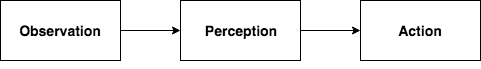
\includegraphics[width=8cm]{drl-pipeline.png}
    }
    \caption{Deep Reinforcement learning end-to-end learning pipeline}
    \label{fig:drl-pipeline}
\end{figure}
